\documentclass[../../../../main.tex]{subfiles}
\begin{document}

\begin{flushright}
\footnotesize\textit{【自動文字起こし・要確認】}
\end{flushright}

\noindent
\textbf{[解]} $g(x) = x^3 - 3x$ とおく. $g'(x) = 3(x+1)(x-1)$ から, 下表を得る.

\begin{center}
\begin{tabular}{c|c|c|c|c|c}
$x$ & $\dots$ & $-1$ & $\dots$ & $1$ & $\dots$ \\ \hline
$g'$ & $+$ & $0$ & $-$ & $0$ & $+$ \\ \hline
$g$ & $\nearrow$ & $2$ & $\searrow$ & $-2$ & $\nearrow$
\end{tabular}
\end{center}

\noindent
したがって, グラフは右図. 題意の解は $y = g(x)$ と $y = p$ の共有点の $x$ 座標に等しい.

\begin{center}
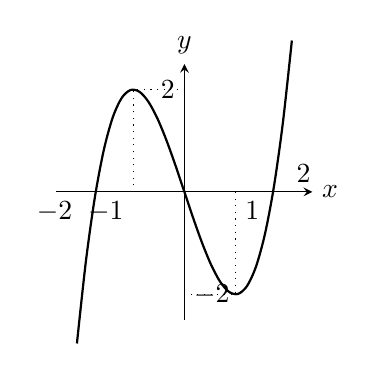
\begin{tikzpicture}[scale=0.65, >=stealth]
\draw[->] (-2.5, 0) -- (2.5, 0) node[right] {$x$};
\draw[->] (0, -2.5) -- (0, 2.5) node[above] {$y$};
\draw[domain=-2.1:2.1, smooth, variable=\x, thick] plot ({\x}, {\x*\x*\x - 3*\x});
\draw[dotted] (-1, 0) -- (-1, 2) -- (0, 2);
\draw[dotted] (1, 0) -- (1, -2) -- (0, -2);
\node[below left] at (-1, 0) {$-1$};
\node[below right] at (1, 0) {$1$};
\node[left] at (0, 2) {$2$};
\node[right] at (0, -2) {$-2$};
\node[below left] at (-2, 0) {$-2$};
\node[above right] at (2, 0) {$2$};
\end{tikzpicture}
\end{center}

\noindent
(1) $|p| > 2$ の時. 図から解はただ 1 つあり, これを $\alpha$ として $f(p) = \alpha^2$ となる. $\alpha^2$ は $|p|$ の単調増加関数であるから, $|p| \to 2$ をかんがえて,
\[
f(p) > 4 \quad \dots \text{①}
\]
以下, 対称性から $0 \le p \le 2$ でかんがえる. $p = 2$ の時, $x = 2, -1$ が解で,
\[
f(p) = -2 \quad \dots \text{②}
\]
となり, $0 < p < 2$ の時, 解は 3 つあり, これを $\alpha, \beta, \gamma$ ($\alpha < \beta < \gamma$) とおく.
\[
\begin{cases}
\alpha + \beta + \gamma = 0 \\
\alpha \beta \gamma = p \\
\beta(\alpha + \gamma) + \alpha \gamma = -3
\end{cases}
\implies
\begin{cases}
-t s = p \\
s - t^2 = -3
\end{cases}
\quad (s = \alpha \gamma, t = \alpha + \gamma) \quad \dots *
\]
から, $f(p) = s = t^2 - 3$ となる. $p = 0$ の時 $t = 0$ となるから, この時 $\min f(p) = -3$ となる. \hfill $\dots$ ③

\noindent
①, ②, ③ から, $\min f(p) = -3$ \quad (又 $f(p) = t^2 - 3$ は $p=2$ でも成立)

\bigskip

\noindent
(2) $y = g(x)$ が奇関数だから, $y = f(p)$ は偶関数である. よって $0 \le p$ でかんがえる.

\medskip
\noindent
$1^\circ \ 0 \le p \le 2$ の時

\noindent
$t$ から, $t = -\beta$ で, $\beta$ は $p$ の単調減少関数だから, $t$ は $p$ の単調増加関数であり, $t = h(p)$ とおくと,
\[
\begin{cases}
h(0) = 0, \quad h(2) = 1 \\
h'(p) > 0
\end{cases}
\]
となり, $0 \le h(p) \le 1$ である.
\[
f'(p) = 2t \frac{dt}{dp} = 2 h(p) \cdot h'(p) > 0 \quad \dots \text{④}
\]
又, $*$ から $s$ を消して
\[
p = -t(t^2 - 3)
\]
だから両辺 $p$ で微分して
\[
1 = -3t^2 \cdot t' + 3t' \quad \therefore \frac{1}{3} = (1 - t^2) \cdot t'
\]
もう1回 $p$ で微分して
\[
0 = t''(1 - t^2) - 2t \cdot (t')^2
\]
$0 \le t \le 1$ から, $0 < p < 2$ では $t' > 0$ となるから, ④より
\[
f''(p) = 2 \{ (t')^2 + t \cdot t'' \} > 0 \quad \dots \text{⑤}
\]
となる. よって ④, ⑤ から, $0 \le p < 2$ では下に凸な単調増加関数である.

\medskip
\noindent
$2^\circ \ 2 < p$ の時

\noindent
唯一の解 $\alpha$ として, $f(p) = \alpha^2$, $p = \alpha^3 - 3\alpha$ だから, $1^\circ$ と同じく $p$ で微分して
\[
1 = (3\alpha^2 - 3)\alpha' \quad \dots \text{⑥}
\]
\[
0 = (\alpha^2 - 1)\alpha'' + 2\alpha(\alpha')^2
\]
となり, $2 < \alpha$ から $\alpha' > 0$ で,
\begin{align*}
f'(p) &= 2\alpha \cdot \alpha' > 0 \\
f''(p) &= 2(\alpha' \cdot \alpha' + \alpha \cdot \alpha'') \\
&= 2 \left\{ (\alpha')^2 + \alpha \frac{-2\alpha(\alpha')^2}{\alpha^2 - 1} \right\} \quad (\because \text{⑥}) \\
&= 2(\alpha')^2 \frac{-(\alpha^2 + 1)}{\alpha^2 - 1} < 0
\end{align*}
となるから, $p > 2$ の時は上に凸な単調増加関数. 又, $f(p) \to +\infty \ (p \to +\infty)$ である.

\noindent
以上からグラフは下図.

\begin{center}
\begin{tikzpicture}[scale=0.8, >=stealth]
\draw[->] (-3.5, 0) -- (3.5, 0) node[right] {$p$};
\draw[->] (0, -3.5) -- (0, 4.5) node[above] {$y$};

\fill (0, -3) circle (2pt) node[below right] {$-3$};

\draw[thick, domain=0:2, smooth] plot (\x, {0.25*\x*\x - 3});
\draw[thick, domain=-2:0, smooth] plot (\x, {0.25*\x*\x - 3});

\draw[dotted] (2, 0) -- (2, -2) -- (0, -2);
\draw[dotted] (-2, 0) -- (-2, -2) -- (0, -2);
\fill (2, -2) circle (2pt);
\fill (-2, -2) circle (2pt);

\node[above] at (2, 0) {$2$};
\node[above] at (-2, 0) {$-2$};
\node[right] at (0, -2) {$-2$};

\draw[thick, domain=2:3.2, smooth] plot (\x, {-2 + 3*sqrt(\x - 2)});
\draw[thick, domain=-3.2:-2, smooth] plot (\x, {-2 + 3*sqrt(-\x - 2)});

\draw[dotted] (-3.5, 4) -- (3.5, 4);
\node[left] at (0, 4) {$4$};
\draw[dotted] (2, 0) -- (2, 4);
\draw[dotted] (-2, 0) -- (-2, 4);
\draw[fill=white] (2, 4) circle (2pt);
\draw[fill=white] (-2, 4) circle (2pt);

\node[below right] at (0,0) {$0$};
\end{tikzpicture}
\end{center}

\end{document}
